% !TEX root = ./main.tex
% Lexical Analysis
% ======================================================
\subsection*{正则表达式和形式语言}
\par \noindent 形式语言的运算:给定语言 $L=\{a, b\}, M = \{cc, dd\}$:
\par \noindent $L \cup M = \{s | s\in L \textor s \in M\} =  \{a, b, cc, dd\}$
\par \noindent $LM = \{st | s\in L \textand t \in M\} = \{acc, add, bcc, bdd\}$
\par \noindent $L^0 = \{\varepsilon\},L^1 = L, L^n = L^{n-1}L^n$
\par \noindent $L^* = L^0 \cup L^1 \cup L^2 \cup \dots$(Kleene 闭包)
\par \noindent $L^+ = L^1 \cup L^2 \cup L^3 \cup \dots$(正闭包)
\par \noindent 运算的优先级:闭包\texttt{*} > 连接 > 选择\texttt{|}
\par \noindent 正则表达式 $r$ 定义正则语言,记为 $L(r)$,正则语言 $L(r), L(s)$:
\par \noindent $L(r|s) = L(r) \cup L(s)$、$L(rs) = L(r)L(s)$、
\par \noindent $L(r^*) = (L(r))^*$、$(L(r)) = (Lr)$
\par \noindent 正则表达式满足运算定律:\texttt{|} 可交换、可结合。连接可结合,对\texttt{|} 可分配。闭包满足幂等性 $r^{**} = r^*$。
\par \noindent FA 无法计数,正则表达式不能用于描述配对或嵌套的结构。
\begin{figure}[H]
    \centering
    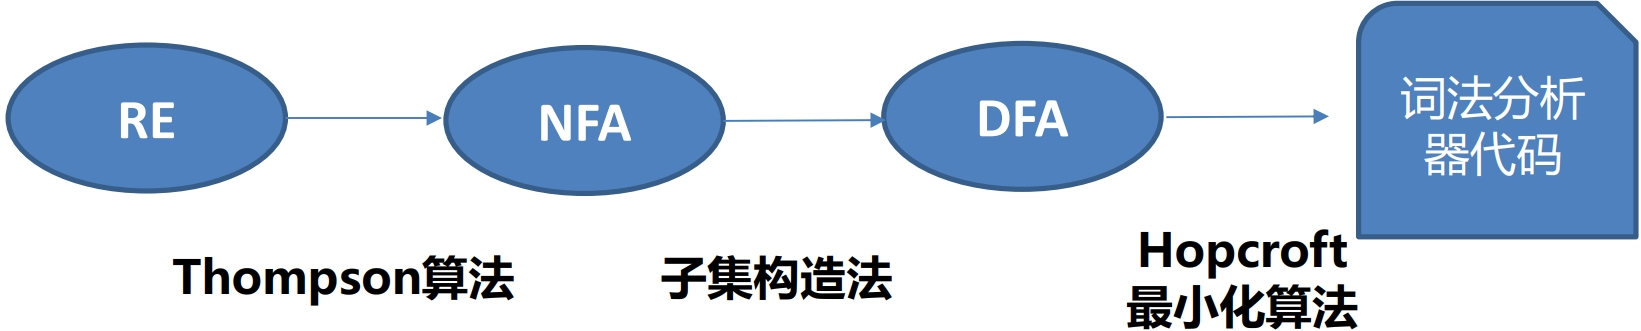
\includegraphics[width=0.8\linewidth]{figures/lex1.png}
\end{figure}
\par \noindent RE $\rightarrow$ NFA:结构归纳法。
\begin{figure}[H]
    \centering
    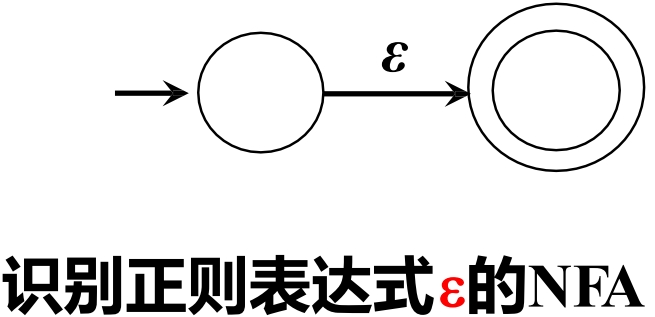
\includegraphics[width=0.3\linewidth]{figures/lex2.png}
    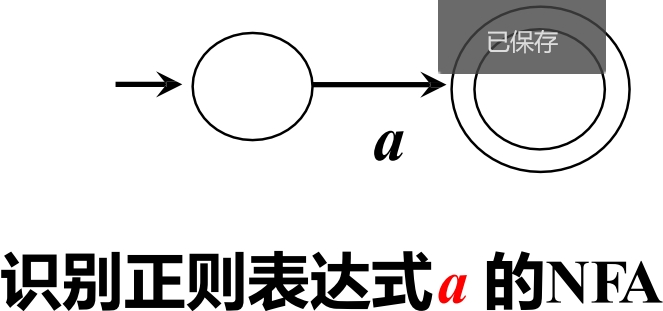
\includegraphics[width=0.3\linewidth]{figures/lex3.png}
    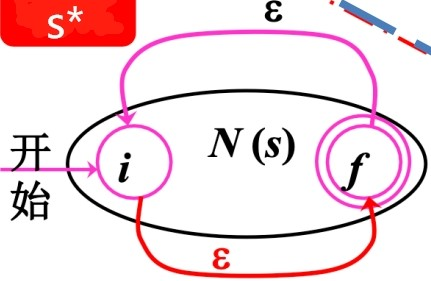
\includegraphics[width=0.2\linewidth]{figures/lex6.png}
\end{figure}
\begin{figure}[H]
    \centering
    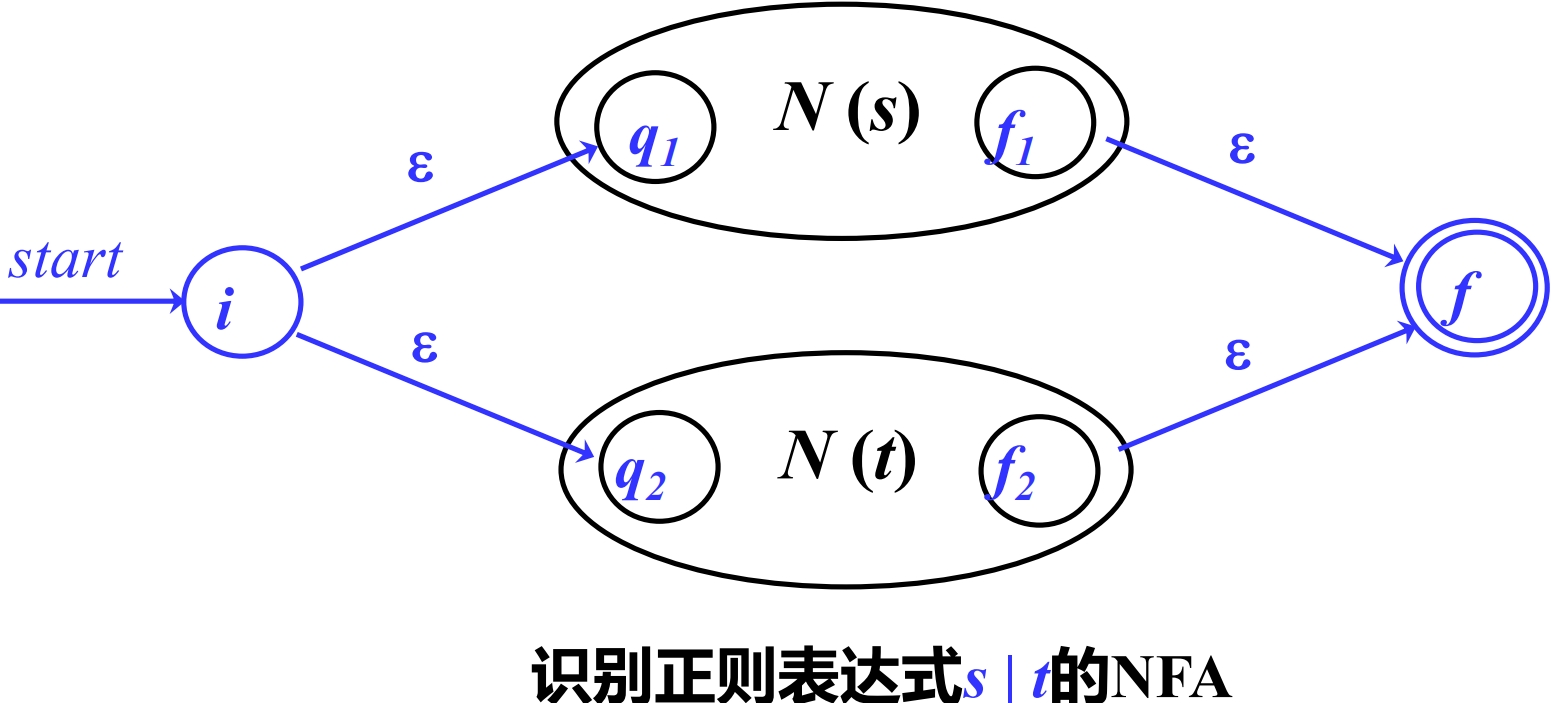
\includegraphics[width=0.4\linewidth]{figures/lex4.png}
    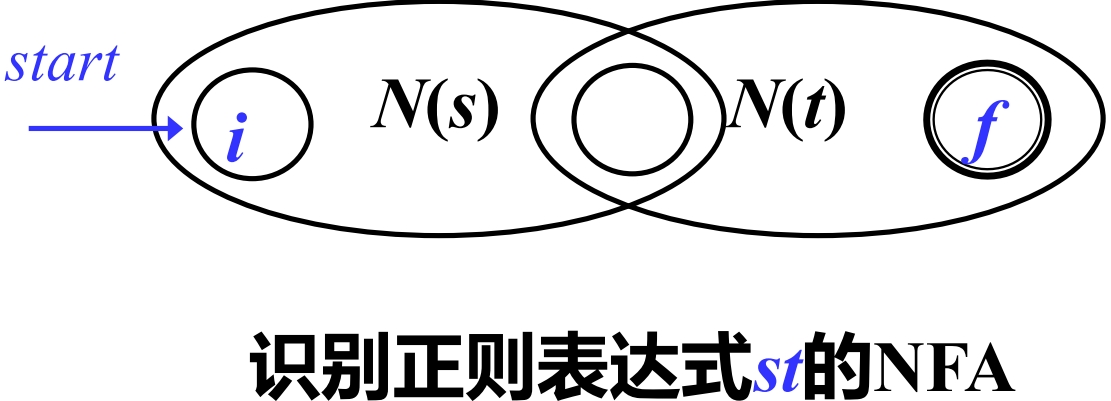
\includegraphics[width=0.4\linewidth]{figures/lex5.png}
\end{figure}
\par \noindent NFA $\rightarrow$ DFA:子集构造法。
\par \noindent NFA 的初始状态的 e-闭包 对应于 DFA 的初始状态。
针对每个 DFA 状态(对应 NFA 状态子集 A ),求输入每个 $a_i$ 后,
能到达的 NFA 状态的 e-闭包 并集 S。
该集合 S 要么对应于 DFA 中的一个已有状态,要么是一个要新加的 DFA 状态,
依据此法,逐步构造 DFA 的状态转换表,直到不动点。
\par \noindent DFA 化简:等价类划分法。
\par \noindent 初始划分:接受状态组和非接受状态组 $\Pi = \{S−F, F\}$,
集合 G 的每个状态读入同一字符后,都落入相同的某个集合,那么就不用细分,否则细分,迭代直到不能细分为止。
% ======================================================
\subsection*{Lex 词法分析工具}
\par Lex 的冲突解决方法:Longest match > Rule Priority。
\begin{figure}[H]
    \centering
    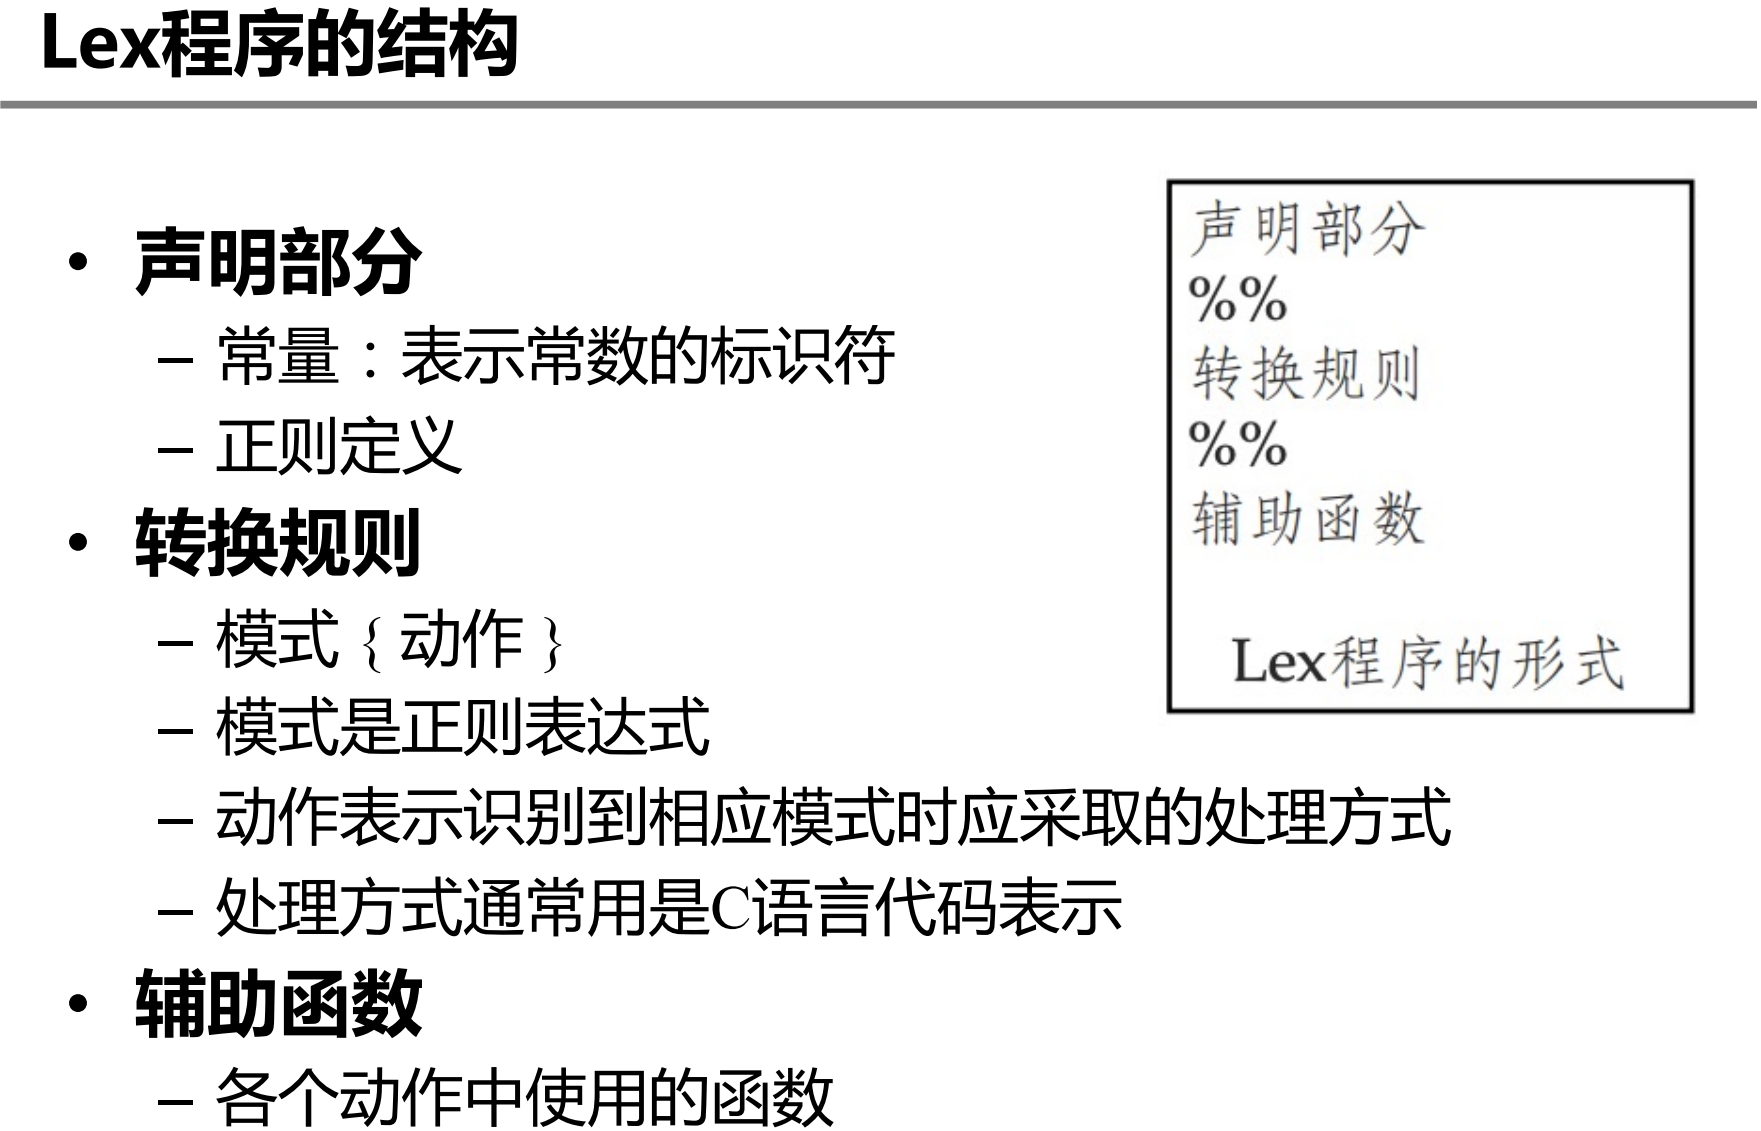
\includegraphics[width=0.4\linewidth]{figures/lex7.png}
    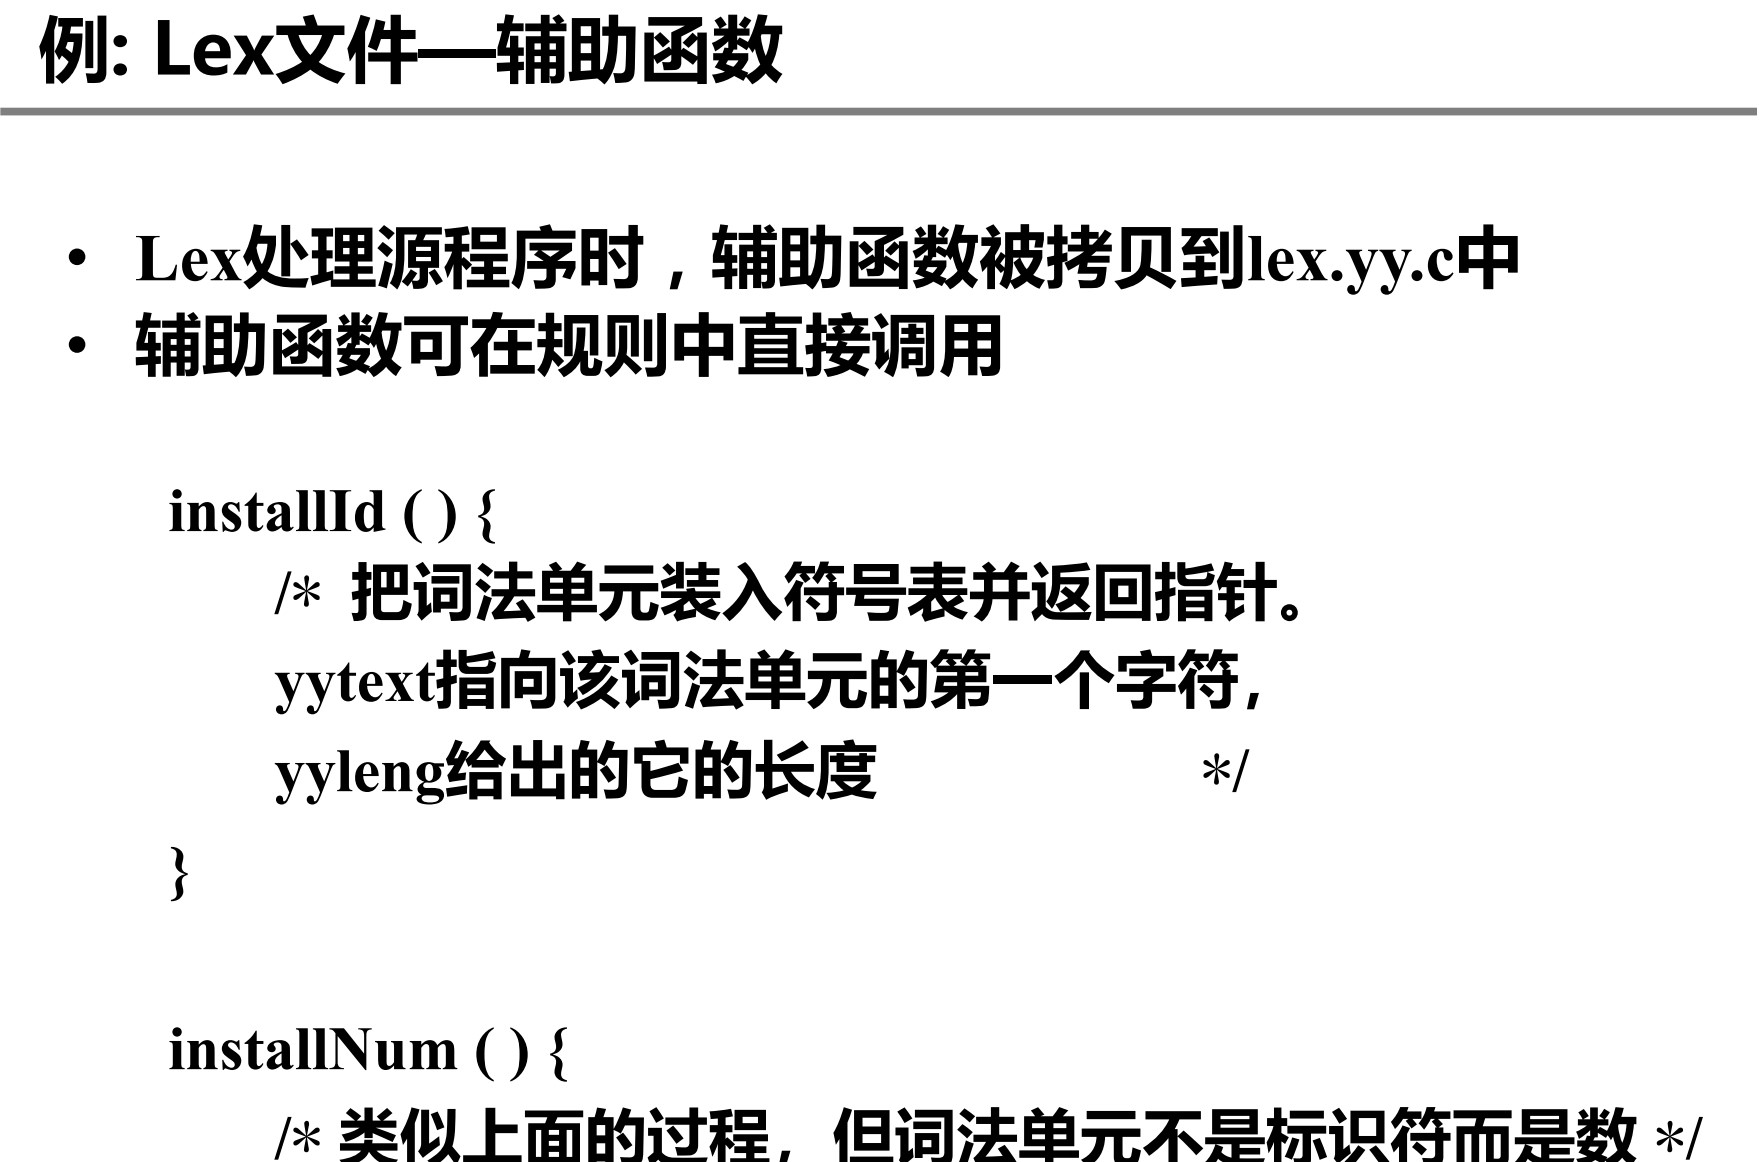
\includegraphics[width=0.4\linewidth]{figures/lex10.png}
    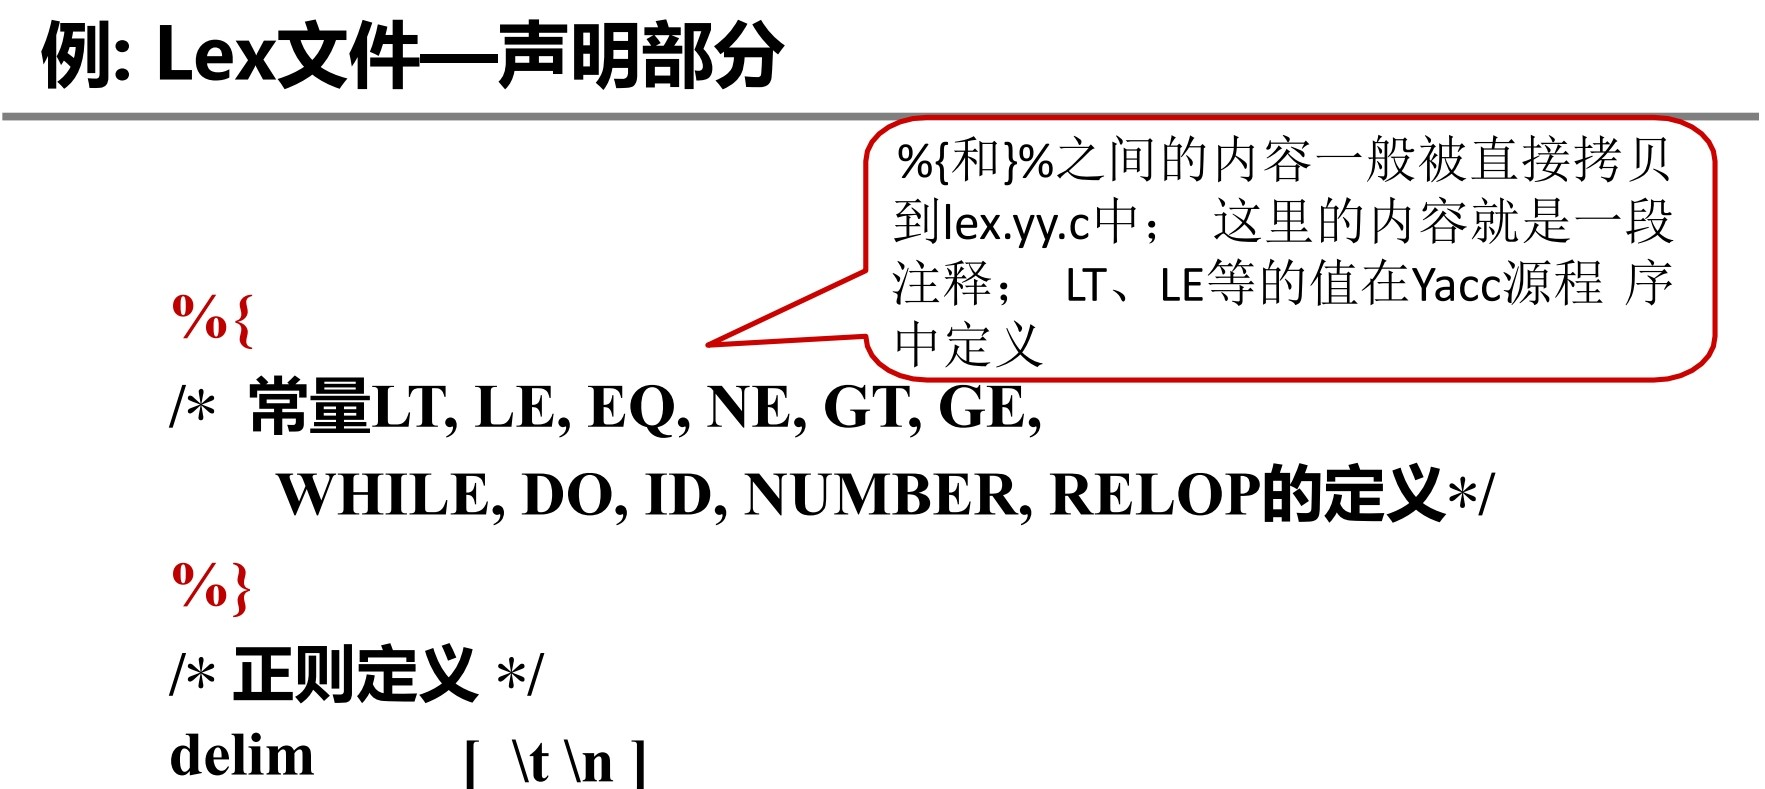
\includegraphics[width=0.4\linewidth]{figures/lex8.png}
    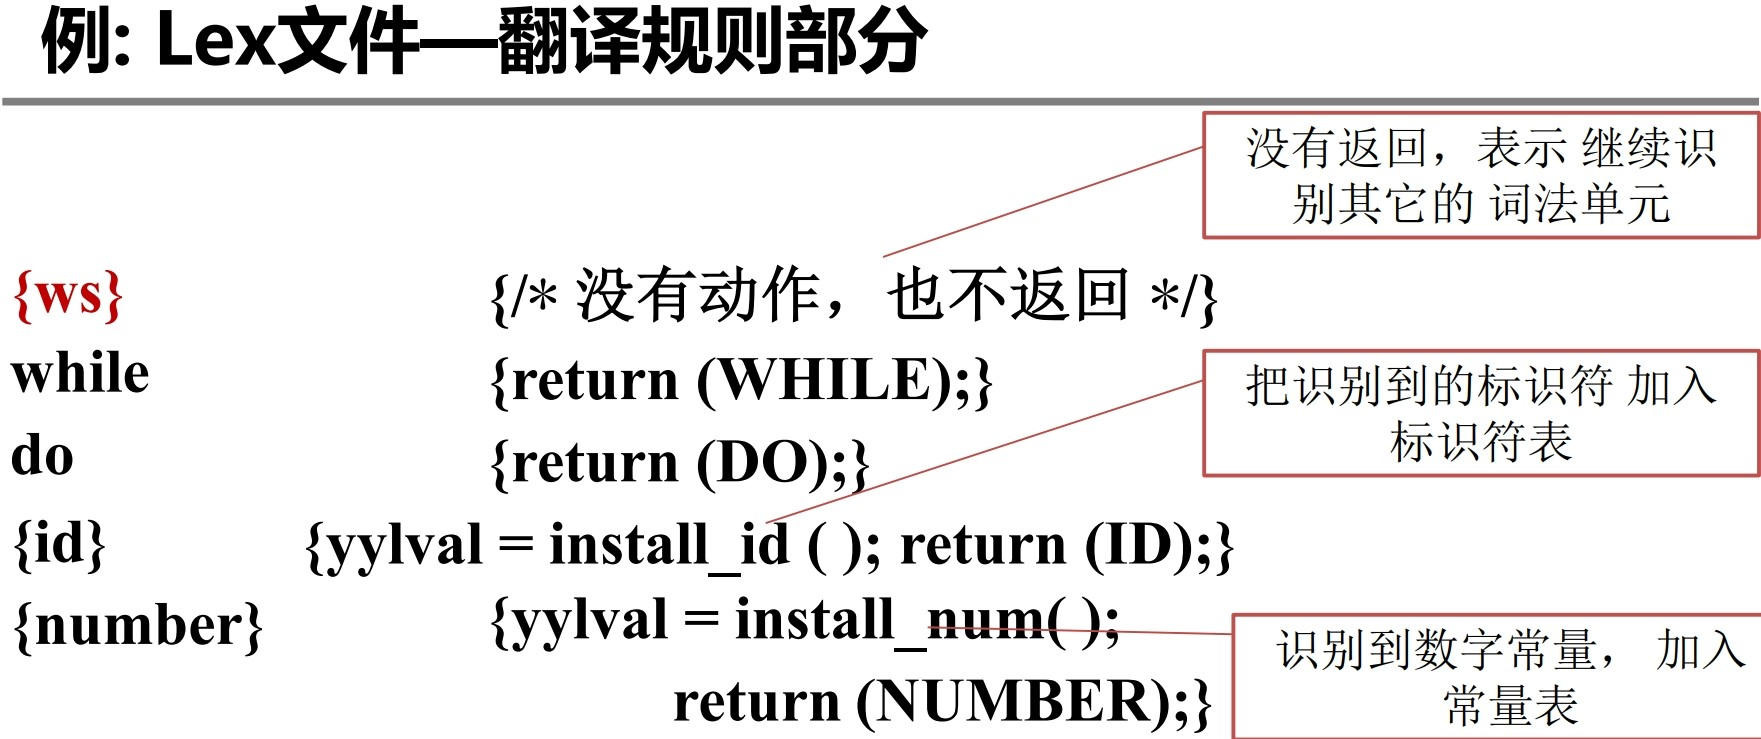
\includegraphics[width=0.4\linewidth]{figures/lex9.png}
\end{figure}
% ======================================================